\begin{frame}
	\frametitle{PITA Scan}
	Run 20621: varied the PITA voltages V1 an V2 together (V1=V2) and measured the asymmetry. Each step corresponds to \approx 60sec of data.
	\begin{columns}
		\column{0.15\textwidth}
		\vspace{12mm}
		\begin{tabular}{|c|}
			\hline
			PITA V1,2 \\\hline
			-9000\\
			-7000\\
			-5000\\
			-3000\\
			-1000\\
			+1000\\\hline
		\end{tabular}
		\column{0.75\textwidth}
		\begin{figure}
			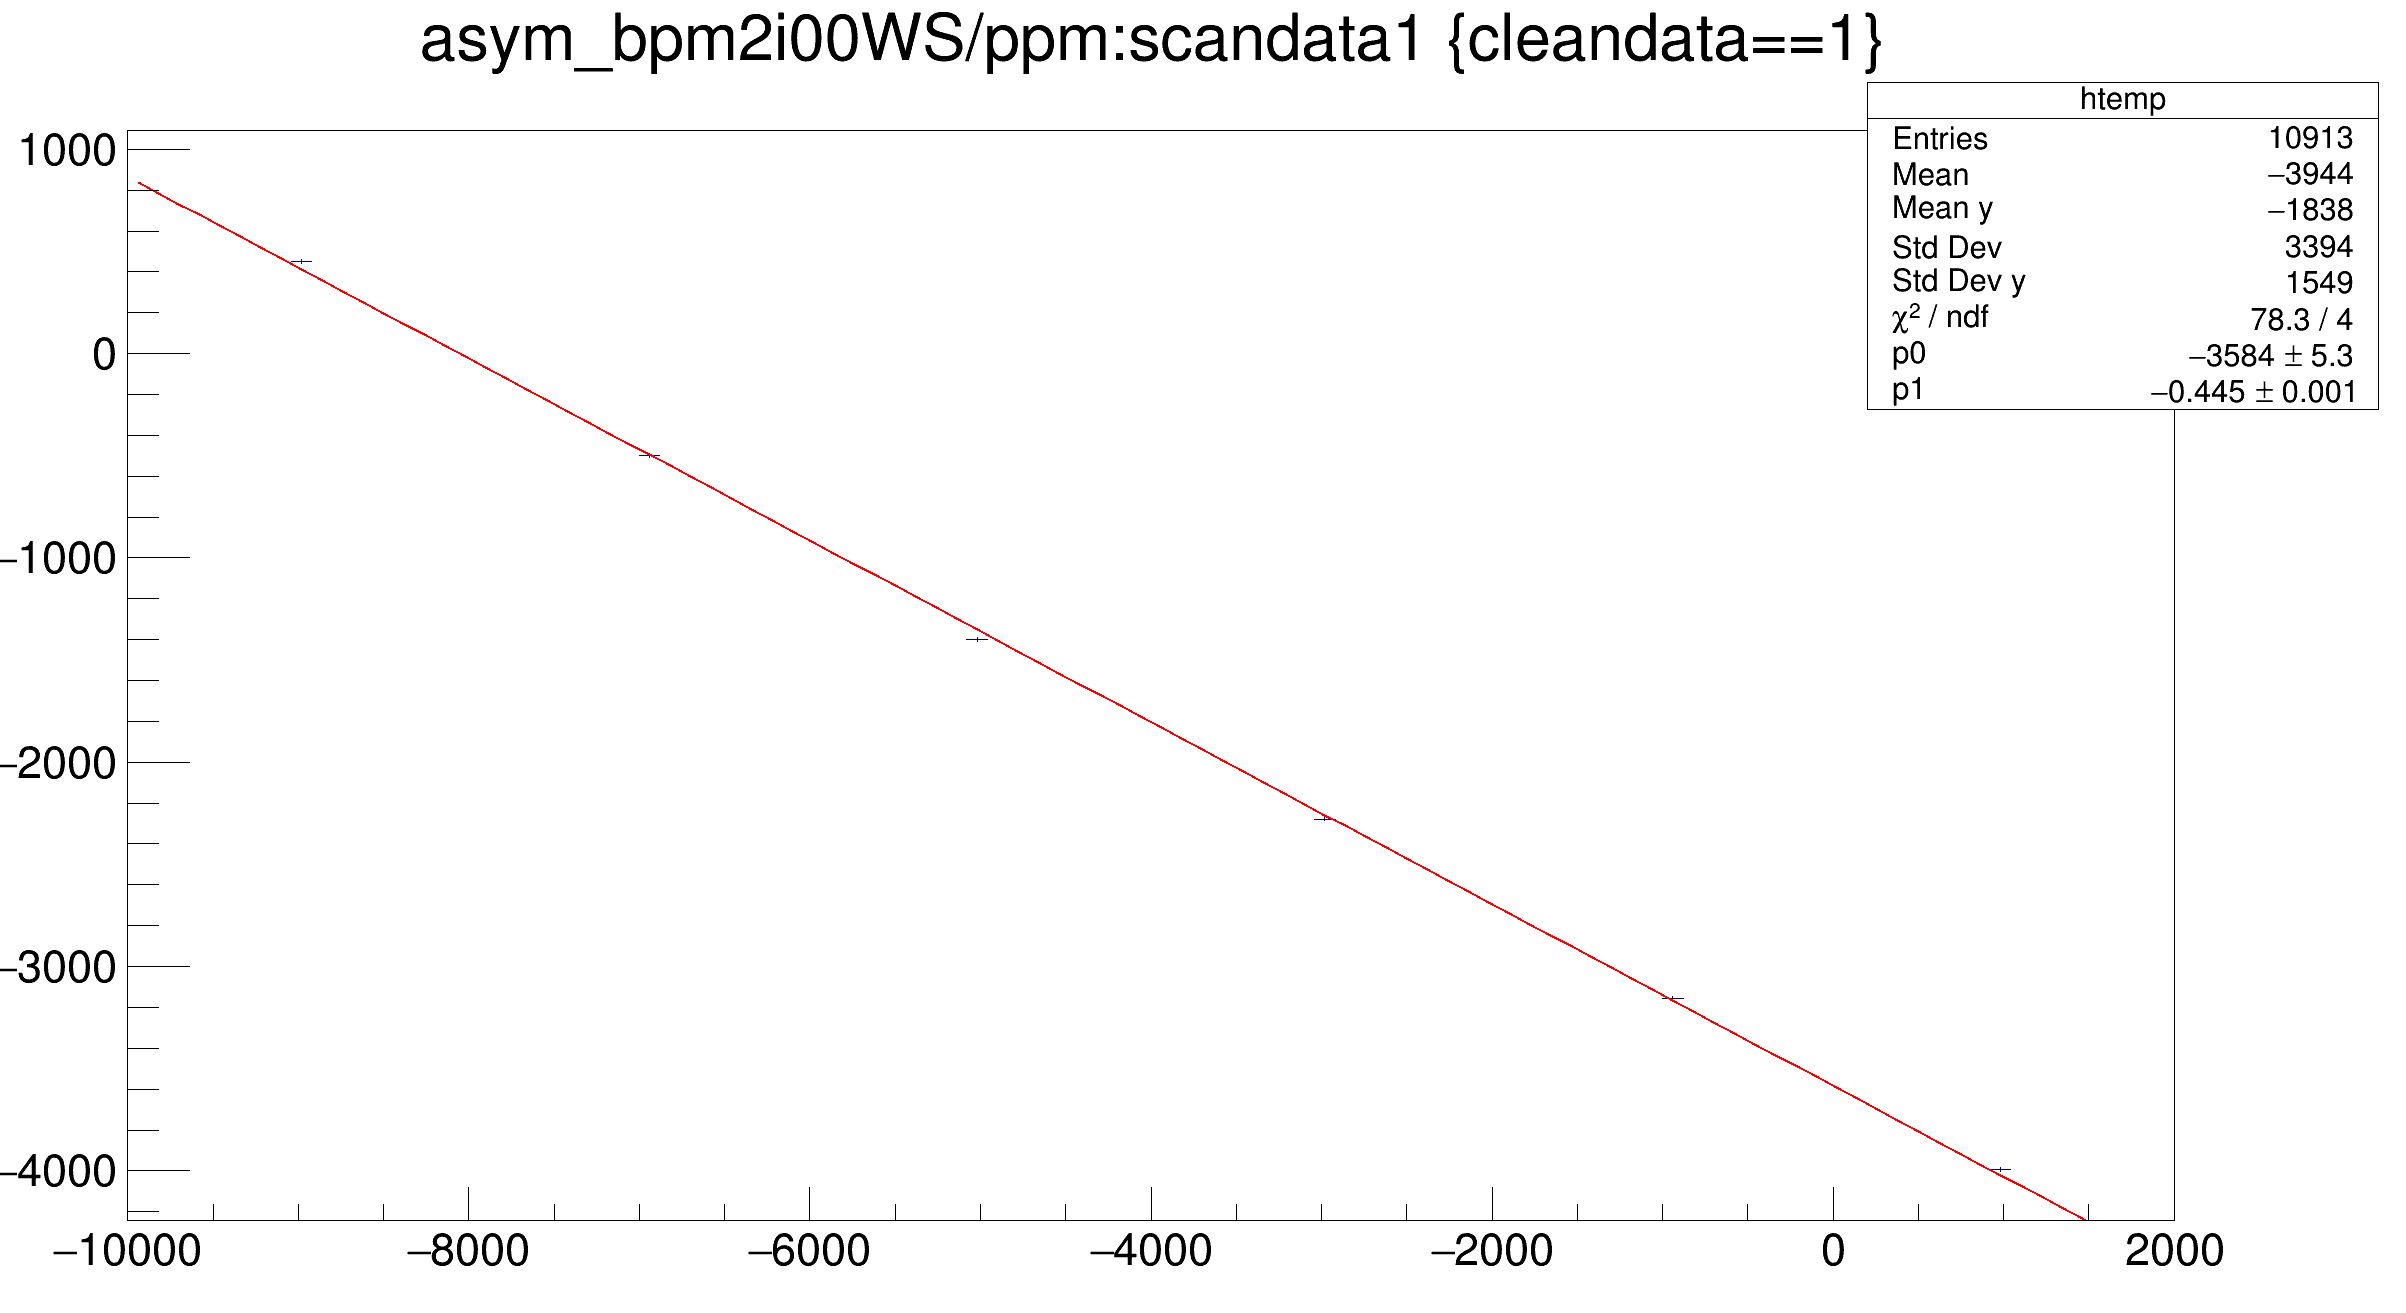
\includegraphics[width=85mm]{./Figs/run20622_pita_slope.png}
		\end{figure}
	\end{columns}
	\vspace{3mm}
	From the fit parameters, we obtained a PITA Voltage of -8054 counts.
\end{frame}